% \chapter{Maintenance}
\chapter{Description des missions}

Dans cette partie je détaillerais avec le plus de précisions possibles les missions que j'ai effectuées. C'est pourquoi j'ai choisi d'examiner chaque missions dans une partie. 

\section{Maintenance}

\subsection{L'organisation de Disneyland}%POS,GFS,Bureautique, les delais, les fax, les SLA ...
\paragraph{}
Un découpage de Disneyland à été établi lors de la création du premier contrat entre la société de service qui s'est occupée de la maintenance du parc et Disneyland.
Ce découpage sert à définir des délais de réparation, mais aussi à simplifier la gestion du stock. En effet, chaque matériel et chaque lieu de Disneyland est affecté à un domaine. Ainsi lorsqu'un problème matériel est déclaré, le technicien sait de quelle délai il dispose pour résoudre le problème.

\newacronym{pos}{POS}{\foreignlanguage{english}{Point Of Sell}}
\newacronym{gfs}{GFS}{Gest Facing System}
\paragraph{}
Il y a trois domaines : \gls{pos}, \gls{gfs}(ou \foreignlanguage{english}{Ticketing}) et Bureautique.
Selon la période de l'année et l'affluence des visiteurs, les délais sont plus ou moins courts.
Le domaine \gls{pos} correspond à tout ce qui touche à la vente de produits dérivés et de consommables. C'est un domaine très important pour la rentabilité du parc. Cependant, d'un point de vu maintenance, ce domaine n'est pas le plus important.
En effet, le domaine \gls{gfs} importe beaucoup plus. Il correspond à tout ce qui à un impact direct avec le visiteur. Par exemple les tourniquets d'entrée du parc, ou les décors font partis de ce domaine. C'est le domaine le plus critique. Il a le délais le plus court. Si un tourniquet reste bloqué à l'entrée du parc, le visiteur sera directement touché. 
Enfin, il y a le domaine bureautique. Ce domaine impact quasiment exclusivement les employés de Disneyland. Il correspond au matériel des employés, comme les imprimantes, les ordinateurs, etc. Il s'agit donc du domaine le moins critique. Nous avons entre 8 et 6 heures pour dépanner le matériel du domaine bureautique.

\paragraph{}
Lorsqu'un employé constate un problème technique sur le matériel, il contact la \foreignlanguage{english}{hotline} et demande un numéro d'intervention. La \foreignlanguage{english}{hotline} de son côté crée un \gls{ot} et l'envoie au service concerné par le problème.
S'il s'agit d'un problème électrique, l'\gls{ot} est transmis à la maintenance électrique, s'il s'agit d'un problème réseau, l'\gls{ot} est transmis à la maintenance réseau, etc...
Notre service s'occupe de la maintenance \gls{hardware}. Tout les \gls{ot} nous sont transmis de deux manières : par fax et via \gls{sm7}. cf. figure~\ref{sm7ListeOt} page~\pageref{sm7ListeOt}.
\begin{center}
  \begin{figure}[ht]
    \caption{\label{sm7ListeOt} SM7}
    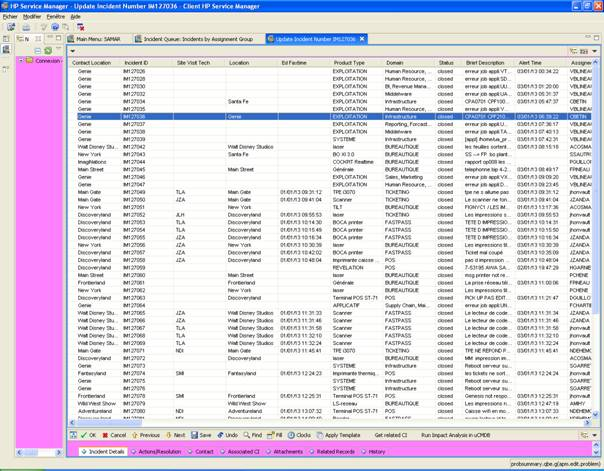
\includegraphics [width=1\textwidth]{images/sm7ListeOt.jpg}
  \end{figure}
\end{center}
Examinons maintenant la façon dont est géré cette \gls{ot} en interne.

\subsection{L'organisation de Spie à Disneyland}%dispatcher, stock, la chef, ...
\paragraph{}
Un fois le fax et l'\gls{ot} reçu, le \gls{dispatcher} effectue un contre-appel afin de s'assurer de la présence de la personne qui a appelé mais aussi pour tenter une réparation par téléphone. Le \gls{dispatcher} peut également prendre des rendez-vous dans le cas où la personne n'est pas disponible dans l’immédiat.
Le \gls{dispatcher} peut alors préparer le matériel dont aura besoin le technicien. Si le matériel doit être changé, alors une sortie de stock doit être effectuée en notant le type de matériel, son ID Disney ainsi que son domaine. Le matériel peut être testé, si le matériel est conditionné. Enfin l'\gls{ot} est assigné à un technicien en fonction du lieu d'intervention et de l'endroit où il se trouve. En effet, si le technicien est déjà en intervention, alors des interventions proches lui seront assignées. 
J'ai pu, durant de courtes périodes, effectuer le travail de \gls{dispatcher}.
Enfin lorsque du matériel revient de réparation, un reparamétrage ou une remasterisation est souvent nécessaire avant de retourner dans le stock. Une intervention en atelier est donc réalisée.
J'ai souvent effectué ce travail en atelier.

Je vais maintenant vous parler de l'intervention sur le terrain de manière plus technique.


\subsection{Le déroulement d'une intervention}%le depart du technicien, le client,...
\paragraph{}
Lorsqu'un technicien débute sa journée, des \gls{ot} lui sont remis sous forme de fax. Après avoir préparé et vérifié son matériel, il part sur le lieu d'intervention en voiture ( même dans les coulisses du parc ). 
Le technicien peut alors réparer le matériel sur place ou bien l'emporter en atelier si nécessaire.

La figure~\ref{st71} page~\pageref{st71} représente une caisse électronique en cours de remasterisation dans l'atelier. Cette remasterisation est une opération très courante, elle résout de nombreux problèmes. J'ai choisi de vous montrer cette réparation comme un exemple car il y a un très grand nombre de matériel différent et donc de problèmes et de solutions différentes. 
Une remasterisation consiste à remettre un "master" (ou un ghost) c'est à dire remettre une image d'un système sur le disque dur d'une caisse. Pour cela on utilise Norton Ghost, sur une clé USB bootable. Ces caisse ne peuvent booter \textbf{que} sur une certaine clé préparé par l'équipe "Customer".
Une fois l'opération terminée, d'autres paramétrages doivent être réalisés, comme par exemple l’ajout d'un pare-feu, l'ajout de certificats pour le wifi, le paramétrage des tiroirs caisse, etc.
\begin{center}
  \begin{figure}[ht]
    \caption{\label{st71} Caisse (ST71) en cours de remasterisation}
    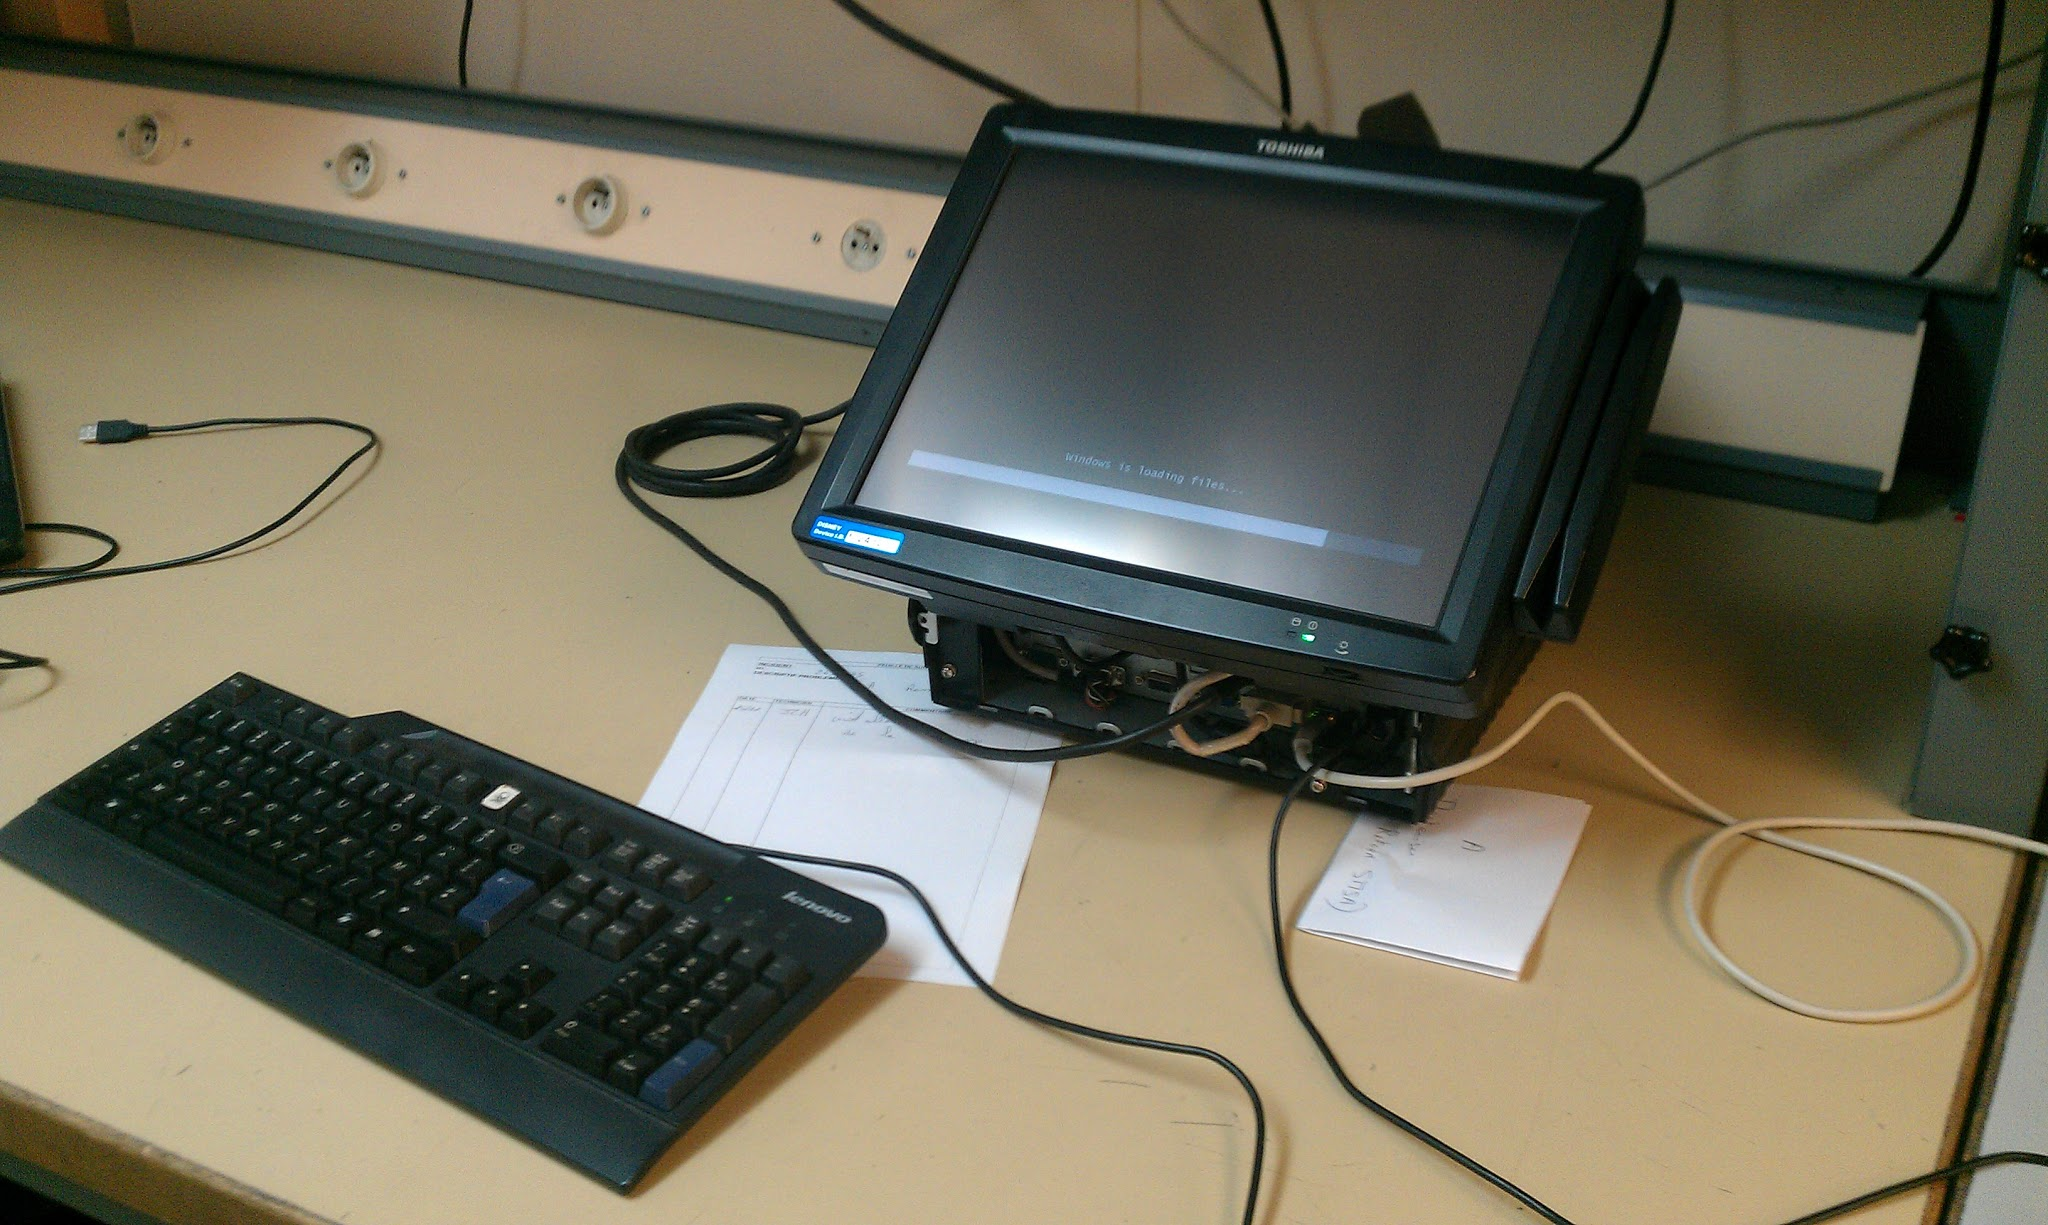
\includegraphics [width=1\textwidth]{images/st71.jpg}
  \end{figure}
\end{center}
\newacronym{ri}{RI}{Rapport d'Intervention}
A la fin d'une intervention, le technicien doit remplir un \gls{ri}, et le faire signer par l'utilisateur du matériel. Ainsi il peut donner le \gls{ri} au \gls{dispatcher} pour clore l'incident. C'est le \gls{dispatcher} qui est chargé de clore les intervention afin que les techniciens gagne du temps.
Pour clore une intervention, le \gls{dispatcher} rempli les champs nécessaires dans \gls{sm7}, et transmet le \gls{ri} au client (Disneyland) après l'avoir scanné et archivé.
